% =====================================================================
% THIS FILE IS THE SOURCE. Edit it, then rebuild the PDF with:
%     bash tools/compile.sh Unit_05_Causal_Thinking
% (run from the Course_Rewrite folder; it compiles twice and reports
%  page count, overfull boxes, and em dashes)
%
% Do not edit the PDF directly. Figures are the fig_*.pdf files in this
% folder, regenerated by tools/make_module*_slide_figs.py.
%
% Originally converted from the 15-module draft by a one-shot script now
% parked in tools/one_shot_generators/. Re-running those would discard
% anything you change here, so they are kept out of tools/ on purpose.
% =====================================================================
\documentclass[aspectratio=169]{beamer}
\usetheme{default}
\usefonttheme{professionalfonts}
\usepackage{amsmath, amssymb, amsfonts}
\usepackage{graphicx}
\usepackage{booktabs}
\usepackage{bm}
\usepackage{hyperref}

\mode<presentation> {
    \usetheme{Frankfurt}
    \usecolortheme{default}
}

\newcommand{\xbar}{\bar{x}}
\newcommand{\yhat}{\hat{y}}

\newenvironment{principle}[1]{\begin{block}{\textbf{Principle:} #1}}{\end{block}}
\newenvironment{trap}[1]{\begin{alertblock}{\textbf{Trap:} #1}}{\end{alertblock}}
\newenvironment{practice}[1]{\begin{exampleblock}{\textbf{In practice:} #1}}{\end{exampleblock}}
\newenvironment{interview}[1]{\begin{exampleblock}{\textbf{You may be asked:} #1}}{\end{exampleblock}}
\newenvironment{yourturn}[1]{%
  \setbeamercolor{block title}{fg=white,bg=orange!80!black}%
  \setbeamercolor{block body}{bg=orange!12}%
  \begin{block}{\textbf{Your turn:} #1}}{\end{block}}
\newenvironment{livedemo}[1]{%
  \setbeamercolor{block title}{fg=white,bg=teal!80!black}%
  \setbeamercolor{block body}{bg=teal!12}%
  \begin{block}{\textbf{Live demo:} #1}}{\end{block}}
\newenvironment{llmcheck}[1]{%
  \setbeamercolor{block title}{fg=white,bg=violet!75!black}%
  \setbeamercolor{block body}{bg=violet!10}%
  \begin{block}{\textbf{LLM check:} #1}}{\end{block}}

\title{Causal Thinking}
\subtitle{Unit 5: From ``What Goes With What'' to ``What Happens If We Change It''}
\author{Stat 220 \textbar{} Statistics for Data Science}
\date{}

\begin{document}

\begin{frame}
  \titlepage
\end{frame}

% ======================================================================
\section{Why}
% ======================================================================
\begin{frame}{Where this fits}
\begin{itemize}
  \item Units 2 through 4 built models, checked them honestly, and predicted with them. Every one
        of those answers an \emph{association} question: given what I see, what do I expect?
  \item Every decision anyone actually needs is a \emph{causal} question: if we change the price,
        send the email, launch the program, what happens?
  \item These are different questions, and no amount of model accuracy converts one into the
        other.
\end{itemize}
\begin{principle}{prediction and intervention are not the same job}
A model can predict rain beautifully from barometer readings. Smashing the barometer does not stop
the rain.
\end{principle}
\end{frame}

\begin{frame}{Live experiment: manufacture a correlation out of nothing}
\begin{livedemo}{everyone roll two dice}
Use real dice, or your phone. Roll \textbf{two} dice and report both numbers, in order.
\begin{itemize}
  \item I will plot every pair on the board. First die on the horizontal axis, second on the
        vertical.
  \item The two rolls are obviously independent. Nobody disputes that.
\end{itemize}
Now: \textbf{keep only the pairs whose sum is 9 or more}, and look at the plot again.
\end{livedemo}
\vspace{0.2em}
{\tiny\textit{Materials: dice, or a phone. Time: 10 minutes.}}
\centering\small Predict, before we do it: what will the relationship look like in the surviving
pairs?
\end{frame}

\begin{frame}{The reveal: selection created a relationship}
\begin{center}
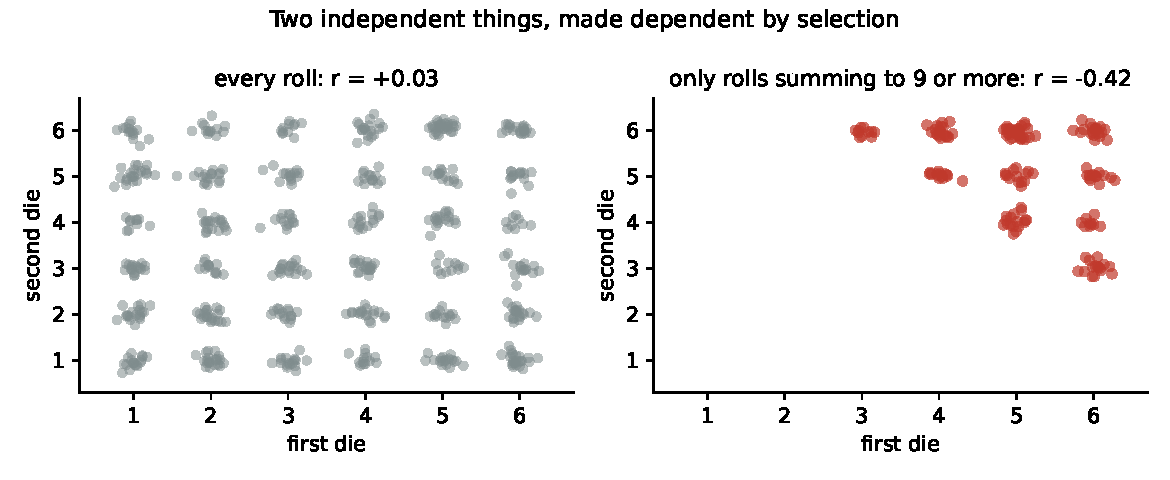
\includegraphics[width=0.92\textwidth]{fig_m12_collider.pdf}
\end{center}
\vspace{-0.4em}
\small
Independent to begin with. Among high-sum rolls, a low first die \emph{requires} a high second
die, so the two become strongly negatively related. Nothing about the dice changed. We changed who
was in the dataset.
\end{frame}

\begin{frame}{Where this shows up in real data}
\begin{itemize}
  \item Restaurants you hear about are either great food or great location, because bad on both
        close. So in your data, food quality and location look negatively related.
  \item Admitted students are either strong on tests or strong on essays. Within the admitted
        class, the two look like they trade off.
  \item Hospitalized patients have some serious condition, so among them, unrelated diseases appear
        connected.
\end{itemize}
\begin{principle}{the sample is part of the analysis}
Before you interpret any relationship, ask who got into the dataset, and what it took to get in.
\end{principle}
\end{frame}

\begin{frame}{What this unit gives you}
\begin{columns}[T]
\begin{column}{0.5\textwidth}
\textbf{Things to know}
\begin{itemize}\small
  \item what a causal effect is, in terms of what would have happened otherwise
  \item why randomization works, and precisely what it buys
  \item what a confounder is, and why you must control for it
  \item what a collider is, and why controlling for it is a disaster
  \item what a mediator is, and when controlling for it answers the wrong question
  \item the main quasi-experimental designs and the assumption each one leans on
\end{itemize}
\end{column}
\begin{column}{0.5\textwidth}
\textbf{Mistakes to stop making}
\begin{itemize}\small
  \item reading a regression coefficient as the effect of intervening
  \item controlling for a collider or for a variable on the causal path
  \item comparing volunteers to non-volunteers and calling it an effect
  \item ignoring who selected into the dataset
  \item treating a before-and-after change as an effect with no control group
  \item forgetting that the treatment might be caused by the outcome
\end{itemize}
\end{column}
\end{columns}
\end{frame}

% ======================================================================
\section{What is an effect}
% ======================================================================
\begin{frame}{An effect is a comparison with something that never happened}
\begin{itemize}
  \item For one customer, the effect of the discount is: what they spend \emph{with} it, minus what
        they would have spent \emph{without} it.
  \item You can only ever observe one of those two. The other is a counterfactual, and it is
        missing by definition.
  \item So causal inference is a \textbf{missing data problem}: everything hinges on how you fill
        in the world that did not happen.
\end{itemize}
\begin{principle}{the question behind every causal claim}
``Compared to what?'' If someone cannot tell you what their comparison group is, they do not have
a causal estimate.
\end{principle}
\end{frame}

\begin{frame}{Why randomization is the gold standard}
\begin{itemize}
  \item Randomly assigning treatment makes the two groups comparable \emph{in expectation} on
        everything: age, motivation, prior spending, and every variable you never thought to
        measure.
  \item That last clause is the important one. Adjustment can only handle confounders you
        measured. Randomization handles the ones you did not.
  \item What it does \emph{not} fix: small samples, dropout after assignment, non-compliance,
        contaminated control groups, or measuring the wrong outcome.
\end{itemize}
\begin{practice}{say this precisely}
``Randomization does not make the groups identical. It makes any difference between them the kind
of difference we can quantify with a standard error.''
\end{practice}
\end{frame}

\begin{frame}{The three roles a third variable can play}
\begin{center}
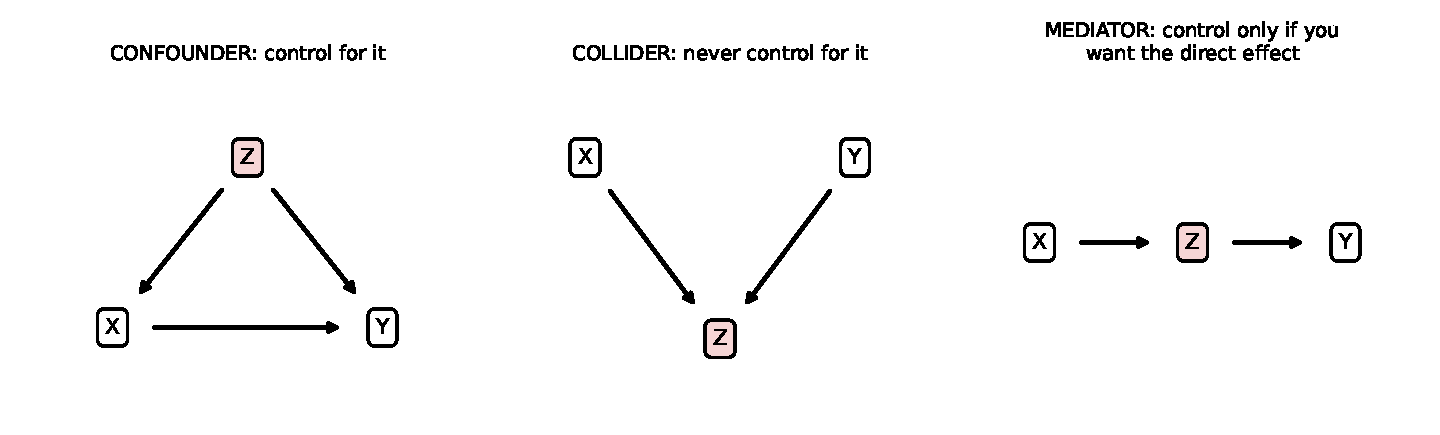
\includegraphics[width=0.98\textwidth]{fig_m12_dags.pdf}
\end{center}
\vspace{-0.2em}
\small
The arrows are what you believe about the world. Which variables to control for is decided by these
diagrams, \emph{not} by which ones improve the fit.
\end{frame}

\begin{frame}{Confounders: the classic problem}
\begin{itemize}
  \item A \textbf{confounder} causes both the treatment and the outcome, producing an association
        with no causal path behind it.
  \item Ice cream sales and drownings both rise with temperature. Neither causes the other.
  \item In business: customers who \emph{choose} the premium plan were already more engaged, so
        premium looks like it causes retention.
\end{itemize}
\begin{principle}{control for confounders, and say which ones you could not measure}
The honest sentence is: ``adjusting for tenure, plan size, and industry, the difference is X, but
I cannot rule out that more motivated teams chose the feature.''
\end{principle}
\end{frame}

\begin{frame}{Confounding in real data}
\begin{center}
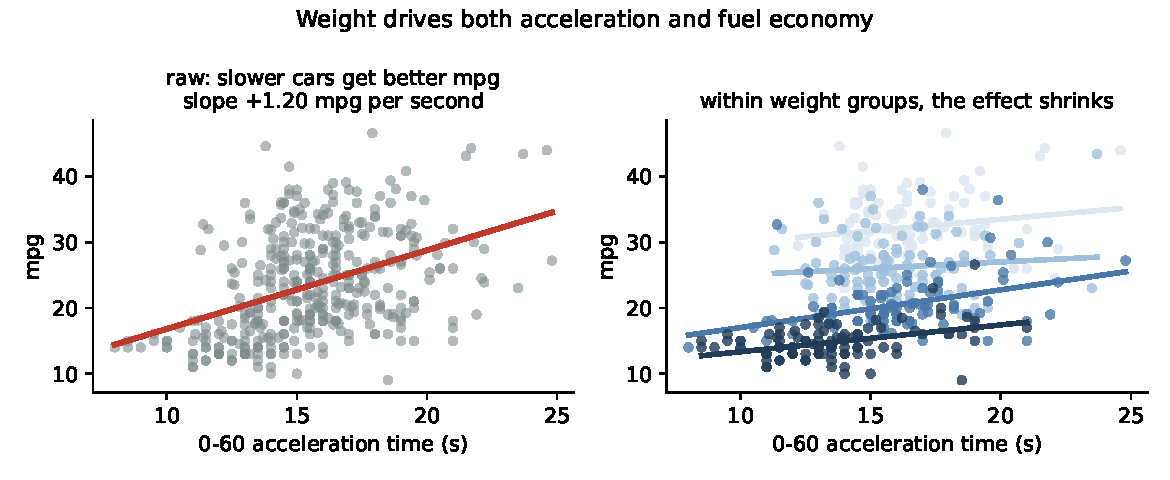
\includegraphics[width=0.9\textwidth]{fig_m12_confounder.pdf}
\end{center}
\vspace{-0.4em}
\small
392 cars. Slower-accelerating cars average \textbf{1.20 mpg better per extra second} to 60. Once
you adjust for weight, which drives both, the association collapses to \textbf{0.26}. Nearly 80\%
of the raw relationship was weight, relabeled.
\end{frame}

\begin{frame}{Colliders: the problem nobody warns you about}
\begin{itemize}
  \item A \textbf{collider} is caused by both variables. Conditioning on it creates an association
        where none existed, exactly as the dice demonstrated.
  \item Selecting your sample on a collider is the same mistake: analyzing only customers who
        \emph{contacted support}, only patients who were \emph{admitted}, only startups that
        \emph{got funded}.
  \item This is why ``add every variable you have to the regression'' is bad advice. Some of those
        variables are colliders, and adding them injects bias rather than removing it.
\end{itemize}
\begin{trap}{the kitchen-sink regression}
More controls is not safer. Each control is a claim about the causal diagram, and the wrong one
makes your estimate worse in a direction you cannot sign.
\end{trap}
\end{frame}

\begin{frame}{Mediators: controlling away the thing you wanted to measure}
\begin{itemize}
  \item A \textbf{mediator} sits on the causal path: training raises skill, skill raises sales.
  \item If you regress sales on training \emph{controlling for skill}, you have removed the very
        channel through which training works, and the effect vanishes.
  \item Controlling for a mediator answers a different, narrower question: is there a direct effect
        \emph{other than} through skill?
\end{itemize}
\begin{practice}{a question that trips people up}
``Should you control for everything?'' The right answer is no, and the reason is exactly this:
confounders yes, colliders never, mediators only if you deliberately want the direct effect.
\end{practice}
\end{frame}

\begin{frame}{The rules, in one table}
\begin{center}\small
\begin{tabular}{p{0.20\textwidth} p{0.30\textwidth} p{0.38\textwidth}}
\toprule
\textbf{Role} & \textbf{Structure} & \textbf{What to do} \\
\midrule
Confounder & causes both $X$ and $Y$ & \textbf{Control for it.} Omitting it biases the
estimate. \\
Collider & is caused by both $X$ and $Y$ & \textbf{Never control for it}, and never select the
sample on it. \\
Mediator & $X$ causes it, it causes $Y$ & \textbf{Leave it out} for the total effect. \\
\bottomrule
\end{tabular}
\end{center}
\vspace{0.4em}
\begin{principle}{the order of operations}
Decide the role from what you believe about the world, \emph{then} write the model. You cannot
read the role off a correlation matrix, and the fit will not tell you either.
\end{principle}
\end{frame}

\begin{frame}{Your turn \#1}
\begin{yourturn}{classify the variable}
You want the effect of a \textbf{new onboarding flow} on 90-day retention. For each variable, say
whether you should control for it, and why:
\begin{enumerate}
  \item Company size at signup.
  \item Number of features used in week one.
  \item Whether the customer contacted support at any point.
\end{enumerate}
\end{yourturn}
\end{frame}

\begin{frame}{Your turn \#1: answer}
\begin{itemize}
  \item \textbf{Company size:} a confounder. It affects both which flow they got (if assignment was
        not random) and retention. \textbf{Control for it.}
  \item \textbf{Features used in week one:} a mediator. That is how onboarding works.
        \textbf{Do not control} unless you specifically want the effect that runs through some
        other channel.
  \item \textbf{Contacted support:} a collider. It is caused by both the onboarding experience and
        by the customer's underlying trouble. \textbf{Never control for it}, and do not restrict
        the sample to those who contacted support.
\end{itemize}
\begin{principle}{draw the arrows before you write the formula}
Two minutes with a diagram prevents a month of arguing about a coefficient.
\end{principle}
\end{frame}

% ======================================================================
\section{When you cannot experiment}
% ======================================================================
\begin{frame}{The realistic situation}
Often you cannot randomize: it is unethical, illegal, too slow, or the change already happened.
Four workhorse designs, each buying credibility with an assumption:
\begin{itemize}
  \item \textbf{Matching / adjustment:} compare treated units to similar untreated ones.
        \emph{Assumes} you measured every confounder.
  \item \textbf{Difference in differences:} compare changes over time against a control group.
        \emph{Assumes} the two groups would have moved in parallel.
  \item \textbf{Regression discontinuity:} compare units just above and just below a cutoff.
        \emph{Assumes} units cannot precisely manipulate their position.
  \item \textbf{Instrumental variables:} use a nudge that affects treatment but nothing else.
        \emph{Assumes} the instrument has no other path to the outcome.
\end{itemize}
\end{frame}

\begin{frame}{Difference in differences, drawn}
\begin{columns}[c]
\begin{column}{0.58\textwidth}
\centering
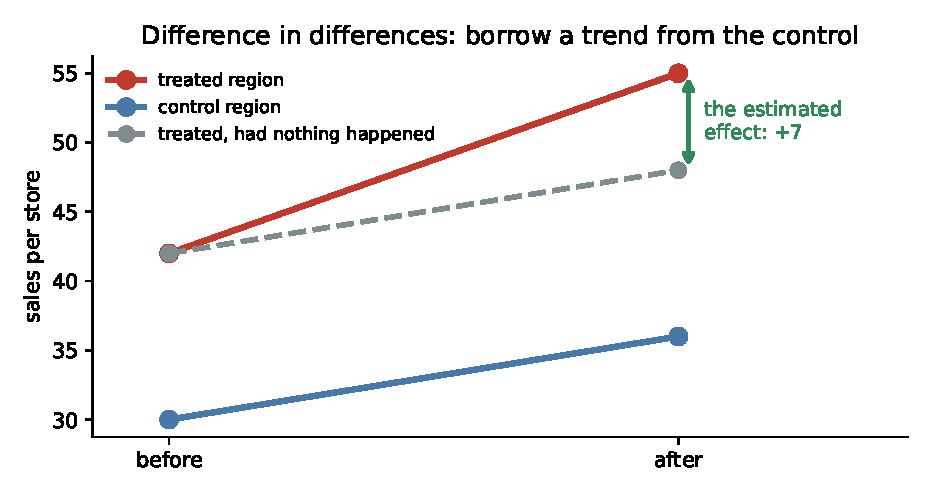
\includegraphics[width=\textwidth]{fig_m12_did.pdf}
\end{column}
\begin{column}{0.42\textwidth}
\small
The treated region rose by 13. But the control region rose by 6 without any treatment, so the
economy was moving anyway.
\begin{itemize}
  \item Estimated effect: $13 - 6 = \textbf{7}$.
  \item Everything rests on the dashed line, the claim that the treated region would have followed
        the control's trend.
\end{itemize}
\end{column}
\end{columns}
\onslide<2->{\centering\small
So the first thing to check is whether the two lines were parallel \emph{before} the change.}
\end{frame}

\begin{frame}{Difference in differences, with the actual arithmetic}
A chain raises pay in its \textbf{Ohio} stores in July and leaves \textbf{Indiana} alone.
\begin{center}\small
\begin{tabular}{lccc}
\toprule
 & \textbf{before} & \textbf{after} & \textbf{change} \\
\midrule
Ohio (treated)    & 42.0 & 55.0 & $+13.0$ \\
Indiana (control) & 30.0 & 36.0 & $+6.0$ \\
\midrule
\textbf{difference in differences} & & & $\mathbf{+7.0}$ \\
\bottomrule
\end{tabular}
\end{center}
\vspace{0.4em}
\begin{itemize}
  \item Ohio rose 13, but 6 of that would have happened anyway. The estimated effect is
        \textbf{7}.
  \item It all rests on the claim that Ohio \emph{would have} risen by 6 too, which is untestable
        after treatment.
\end{itemize}
\begin{principle}{how to check what you cannot test}
Plot both series for several periods \emph{before} the change. If they moved together then, the
assumption is credible.
\end{principle}
\end{frame}

\begin{frame}{Reverse causation, and how to rule it out}
\begin{itemize}
  \item Hospitals with more staff have higher mortality. Do nurses kill people, or do sicker
        patients get more nurses?
  \item Ad spend and sales move together, partly because budgets are \emph{set} as a percentage of
        expected sales.
  \item Police numbers and crime, tutoring and grades, maintenance and failures: in each case the
        outcome plausibly causes the treatment.
\end{itemize}
\begin{principle}{the fix is timing, not statistics}
Establish that the cause moved \emph{first}, and for a reason unrelated to the outcome. That is
what a rollout date, a policy change, or a budget freeze gives you, and no regression can
substitute for it.
\end{principle}
\end{frame}

\begin{frame}{Natural experiments worth knowing}
\begin{itemize}
  \item \textbf{John Snow, 1854:} two water companies served interleaved houses on the same London
        streets, one drawing from sewage-contaminated water. The houses were otherwise alike, so
        the cholera difference was as good as randomized.
  \item \textbf{Minimum wage, 1994:} Card and Krueger compared fast-food employment in New Jersey
        after a wage increase against neighboring Pennsylvania, a difference in differences that
        reversed the textbook prediction.
  \item \textbf{Scholarship cutoffs:} students just above and just below a score threshold are
        nearly identical, so the cutoff acts like a coin flip.
\end{itemize}
\begin{principle}{look for the accident}
The best observational studies find a moment where something outside the actors' control assigned
the treatment for them.
\end{principle}
\end{frame}

\begin{frame}{Your turn \#2}
\begin{yourturn}{design the study}
Your company rolled out a new sales-training program. Reps who completed it sold 18\% more last
quarter than reps who did not. Leadership wants to make it mandatory.
\vspace{0.3em}

With a neighbor: name two reasons that 18\% may not be the effect of training, and design a study
you could actually run next quarter.
\end{yourturn}
\end{frame}

\begin{frame}{Your turn \#2: answer}
\begin{itemize}
  \item \textbf{Selection:} reps who volunteered were more motivated, and would have improved
        anyway. \textbf{Regression to the mean:} if struggling reps were assigned, expect a bounce
        with no cause.
  \item \textbf{Timing:} the quarter may have been better for everyone, which a simple before-after
        comparison would credit to training.
  \item \textbf{The study:} randomize the next cohort. If that is impossible, use a staged rollout
        by region and compare with difference in differences, checking that the regions were
        parallel beforehand.
\end{itemize}
\begin{principle}{staged rollouts are free experiments}
If you must launch to everyone eventually, launch in a random order. It costs nothing and converts
a guess into an estimate.
\end{principle}
\end{frame}

% ======================================================================
\section{LLM check}
% ======================================================================
\begin{frame}{Your turn \#3}
\begin{yourturn}{sort the variables}
You want the effect of a \textbf{price increase} on \textbf{customer churn}. For each variable,
say confounder, collider, or mediator, and whether it belongs in the model:
\begin{enumerate}
  \item The customer's contract tier, which affects both the price they were offered and their
        likelihood of leaving.
  \item Whether the customer called support to complain about the price.
  \item How much the customer's monthly bill actually rose.
\end{enumerate}
\end{yourturn}
\end{frame}

\begin{frame}{Your turn \#3: answer}
\begin{itemize}
  \item \textbf{Contract tier: confounder.} It drives both the treatment and the outcome, so
        leaving it out biases the estimate. \textbf{Control for it.}
  \item \textbf{Complaint call: collider.} It is caused by the price increase \emph{and} by the
        customer's underlying unhappiness. Controlling for it, or studying only complainers,
        manufactures a relationship. \textbf{Leave it out.}
  \item \textbf{Size of the bill increase: mediator.} It is how the price increase acts. Include
        it only if you specifically want the effect of price that runs through something else.
\end{itemize}
\begin{principle}{how to spot it}
Ask ``did this happen before or after the treatment?'' Anything measured afterward is a candidate
mediator or collider, and both are dangerous controls.
\end{principle}
\end{frame}

\begin{frame}{LLM check: mistake or not? (1 of 2)}
\begin{llmcheck}{we asked an LLM about a feature launch}
\textbf{We told it:} ``Customers who use our new dashboard renew at 91\%, others at 68\%. What is
the effect of the dashboard on renewal?''\\[4pt]
\textbf{It answered:} ``The dashboard increases renewal by 23 percentage points. To be thorough I
would control for every variable available in your database to remove any confounding.''
\end{llmcheck}
\vspace{0.2em}
\centering\small Mistake, or no mistake?
\onslide<2->{%
\begin{trap}{verdict: mistake, twice}
First, the 23 points is a comparison between customers who \emph{chose} the dashboard and those who
did not, so it is mostly selection. Second, ``control for everything'' is wrong: some of those
variables are colliders and mediators, and controlling for them adds bias.
\end{trap}}
\end{frame}

\begin{frame}{LLM check: mistake or not? (2 of 2)}
\begin{llmcheck}{same territory, a different answer}
\textbf{We told it:} ``Our ad spend and sales are correlated at 0.8 across 24 months. Does
advertising drive sales?''\\[4pt]
\textbf{It answered:} ``Not necessarily. Ad budgets are often set as a percentage of expected
sales, so sales may be causing spend. Both also rise in the holiday season, which is a confounder.
I would look for a period when spend changed for a reason unrelated to sales, such as a budget
freeze or a regional rollout, and compare against a similar region.''
\end{llmcheck}
\vspace{0.2em}
\centering\small Mistake, or no mistake?
\onslide<2->{%
\begin{principle}{verdict: no mistake}
It raised reverse causation, named a confounder, and proposed a design. That is the full causal
checklist in three sentences.
\end{principle}}
\end{frame}

% ======================================================================
\section{Workflow}
% ======================================================================
\begin{frame}{How to answer ``does X cause Y?''}
\begin{enumerate}
  \item \textbf{State the intervention precisely.} Who gets what, instead of what?
  \item \textbf{Name the comparison group.} If there is none, stop.
  \item \textbf{Draw the diagram}: candidate confounders, colliders, mediators.
  \item \textbf{Ask how treatment was assigned.} Randomized, chosen, or assigned by a rule?
  \item \textbf{Choose the design} that fits the assignment mechanism.
  \item \textbf{Check the design's assumption} explicitly (parallel pre-trends, balance, no
        manipulation at the cutoff).
  \item \textbf{Report the effect with its uncertainty and its caveats}, including the confounder
        you could not measure.
\end{enumerate}
\end{frame}

\begin{frame}{Scenario: the loyalty program that ``worked''}
\textbf{Setup.} Members of a new loyalty program spend \$340 a year. Non-members spend \$180.
Marketing claims the program doubled spending.
\begin{itemize}
  \item Who joins a loyalty program? People who already shop there often. The comparison is between
        heavy and light customers, not between two versions of the same customer.
  \item Adjusting for prior-year spending would help, but only if you have it, and it will not
        remove intent.
  \item The clean answer: randomize invitations, or use a staged geographic rollout, and compare
        the change in spending, not the level.
\end{itemize}
\begin{interview}{how to answer}
``The 160-dollar gap is mostly selection. I would estimate this from a randomized invitation, and I
would look at the change in spending rather than its level.''
\end{interview}
\end{frame}

% ======================================================================
\section{Consolidate}
% ======================================================================
\begin{frame}{Answering ``does X cause Y?''}
\small
\begin{enumerate}
  \item \textbf{State the intervention precisely.} Who gets what, instead of what?
  \item \textbf{Name the comparison group.} If there is none, stop.
  \item \textbf{Draw the diagram} and classify every candidate control as confounder, collider, or mediator.
  \item \textbf{Ask how treatment was assigned}: randomized, self-selected, or by a rule?
  \item \textbf{Choose the design that matches the assignment}, and write down the assumption it buys.
  \item \textbf{Check that assumption explicitly}, for example by plotting pre-treatment trends.
  \item \textbf{Report the estimate, its uncertainty, and the confounder you could not measure.}
\end{enumerate}
\end{frame}

\begin{frame}{The traps, all in one place}
\begin{trap}{the ones that bite most often}
\begin{itemize}
  \item Reading a regression coefficient as the effect of intervening.
  \item Controlling for everything you have.
  \item Conditioning on a collider, including by how you selected the sample.
  \item Controlling for a mediator and reporting the shrunken effect as ``no effect.''
  \item Comparing volunteers to non-volunteers.
  \item Treating a before-after change as an effect with no control group.
  \item Forgetting that the treatment might be caused by the outcome.
\end{itemize}
\end{trap}
\end{frame}

\begin{frame}{Ten questions to be able to answer}
\begin{enumerate}\small
  \item Users of feature X retain better. Should we push everyone onto it?
  \item Why does randomization work, and what does it fail to fix?
  \item Should you control for every variable you have? Explain with an example.
  \item What is a collider, and give a case where selecting on one misled someone?
  \item When would controlling for a variable be actively harmful?
  \item We cannot run an experiment. What are the options, and what does each assume?
  \item How would you check the parallel-trends assumption?
  \item Ad spend and sales correlate at 0.8. What do you conclude?
  \item Our program's participants improved 18\%. What do you ask first?
  \item How would you design a rollout so it produces a causal estimate for free?
\end{enumerate}
\end{frame}

\begin{frame}{Mastery checklist}
You have this unit when you can, from memory:
\begin{itemize}
  \item define a causal effect as a comparison with a counterfactual
  \item explain precisely what randomization buys and what it does not
  \item classify a variable as confounder, collider, or mediator and act accordingly
  \item explain why ``control for everything'' is wrong
  \item name four quasi-experimental designs and the assumption behind each
  \item design a staged rollout that yields a defensible estimate
\end{itemize}
\end{frame}

\begin{frame}{What you should be able to do with software}
\small
Nobody is asking you to memorize syntax. You are expected to know \emph{which} procedure the
question calls for, what to hand it, and what the output means. With an AI assistant open, you
should be able to produce any of these and defend the result.
\begin{center}\footnotesize
\begin{tabular}{p{0.44\textwidth} p{0.46\textwidth}}
\toprule
\textbf{You should be able to} & \textbf{What you would reach for} \\
\midrule
Adjusted comparison & \texttt{smf.ols(\"y \textasciitilde\ treat + covariates\", data)} \\
Estimates within strata & \texttt{pd.qcut} then \texttt{groupby} \\
Difference in differences & four group means, then the difference of the differences \\
Check parallel pre-trends & plot both series for several periods before treatment \\
Randomized assignment for a rollout & \texttt{rng.integers(0, 2, n)} on the unit of assignment \\
Simulate a confounder or a collider & generate the data yourself and compare estimates \\
Logistic version for a binary outcome & \texttt{smf.logit} \\
\bottomrule
\end{tabular}
\end{center}
\vspace{0.2em}
\centering\small
If you cannot say what the output means, the fact that you produced it is worth nothing.
\end{frame}

\begin{frame}{Where we go next}
\begin{itemize}
  \item We have been treating the data as the only source of information. \textbf{Unit 12} lets
        prior knowledge enter the estimate explicitly, and makes decisions by weighing outcomes
        rather than by rejecting a null.
\end{itemize}
\begin{principle}{the through-line}
The data can only tell you what went with what. The causal claim comes from the design, and the
design is your job.
\end{principle}
\end{frame}

\end{document}
